\section*{3. \"Ubung (Abgabe: 28.04.2010, 8.30 Uhr, schriftlich)}

\subsection*{1. Berechnen Sie $z_{1}+z_{2}, z_{1}-z_{2}, z_{2}-z_{1}, z_{1}\cdot z_{2}, z_{1}/z_{2}, z_{1}^{*}\cdot z_{2}, z_{1}/z_{2}^{*}$ f\"ur}
Siehe Tabelle \ref{tab:3.1}.

%% LyX 1.6.5 created this file.  For more info, see http://www.lyx.org/.
%% Do not edit unless you really know what you are doing.

%%%%%%%%%%%%%%%%%%%%%%%%%%%%%% LyX specific LaTeX commands.
%% Because html converters don't know tabularnewline
\providecommand{\tabularnewline}{\\}

%
\begin{table}[h]
\begin{centering}
\begin{tabular}{|c|c|}
\hline 
 & $z_{1}=4-5j,z_{2}=4+5j$\tabularnewline
\hline
\hline 
$z_{1}+z_{2}$ & $8$\tabularnewline
\hline 
$z_{1}-z_{2}$ & $-10j$\tabularnewline
\hline 
$z_{2}-z_{1}$ & $10j$\tabularnewline
\hline 
$z_{1}\cdot z_{2}$ & $41$\tabularnewline
\hline 
$z_{1}/z_{2}$ & $-1-j\frac{40}{41}$\tabularnewline
\hline 
$\overline{z_{1}}\cdot z_{2}$ & $41+j40$\tabularnewline
\hline 
$z_{1}/\overline{z_{2}}$ & $1$\tabularnewline
\hline
\end{tabular}
\par\end{centering}
\caption{L\"osungen zu 3.1}
\label{tab:3.1}
\end{table}




\subsection*{2. Gegeben sei eine periodische Funktion \"uber die Zeit, wie lauten die Koeffizienten der \emph{komplexen} Fourierreihe?}
a) $f(t) = \sin(t)~\text{f\"ur}~t \in (-\pi, \pi)$\\
$a_0 = 0; ~ c_{1} = -\frac{1}{2}j; ~ \bar{c_{1}} = \frac{1}{2}j;$\\\\
b) $f(t) = \cos(t)~\text{f\"ur}~t \in (-\pi, \pi)$\\
$a_0 = 0; ~ c_{1} = \frac{1}{2} = \bar{c_{1}};$\\\\
c) $f(t) = \cos(2t)~\text{f\"ur}~t \in (-\pi, \pi)$\\
$a_0 = 0; ~ c_{2} = \frac{1}{2} = \bar{c_{2}};$\\\\
d) $f(t) = 1~\text{f\"ur}~t \in (-\pi, \pi)$\\
$a_0 = 2; ~ c_{k} = 0 = \bar{c_{k}};$\\\\
e)$f(t)=sin(t)+cos(t)~\text{f\"ur}~t \in (-\pi, \pi)$\\
$a_0 = 0; ~ c_{1} = \frac{1}{2}(1-j); ~ \bar{c_{1}} = \frac{1}{2}(1+j);$\\\\

\subsection*{3. Gegeben seien die Fourierkoeffizienten einer Funktion \"uber die Zeit. Wie lautet die Funktion?}
Siehe Abbildungen \ref{fig:3.3.a},  \ref{fig:3.3.b}.
\begin{figure}[h] %  figure placement: here, top, bottom, or page
   \centering
   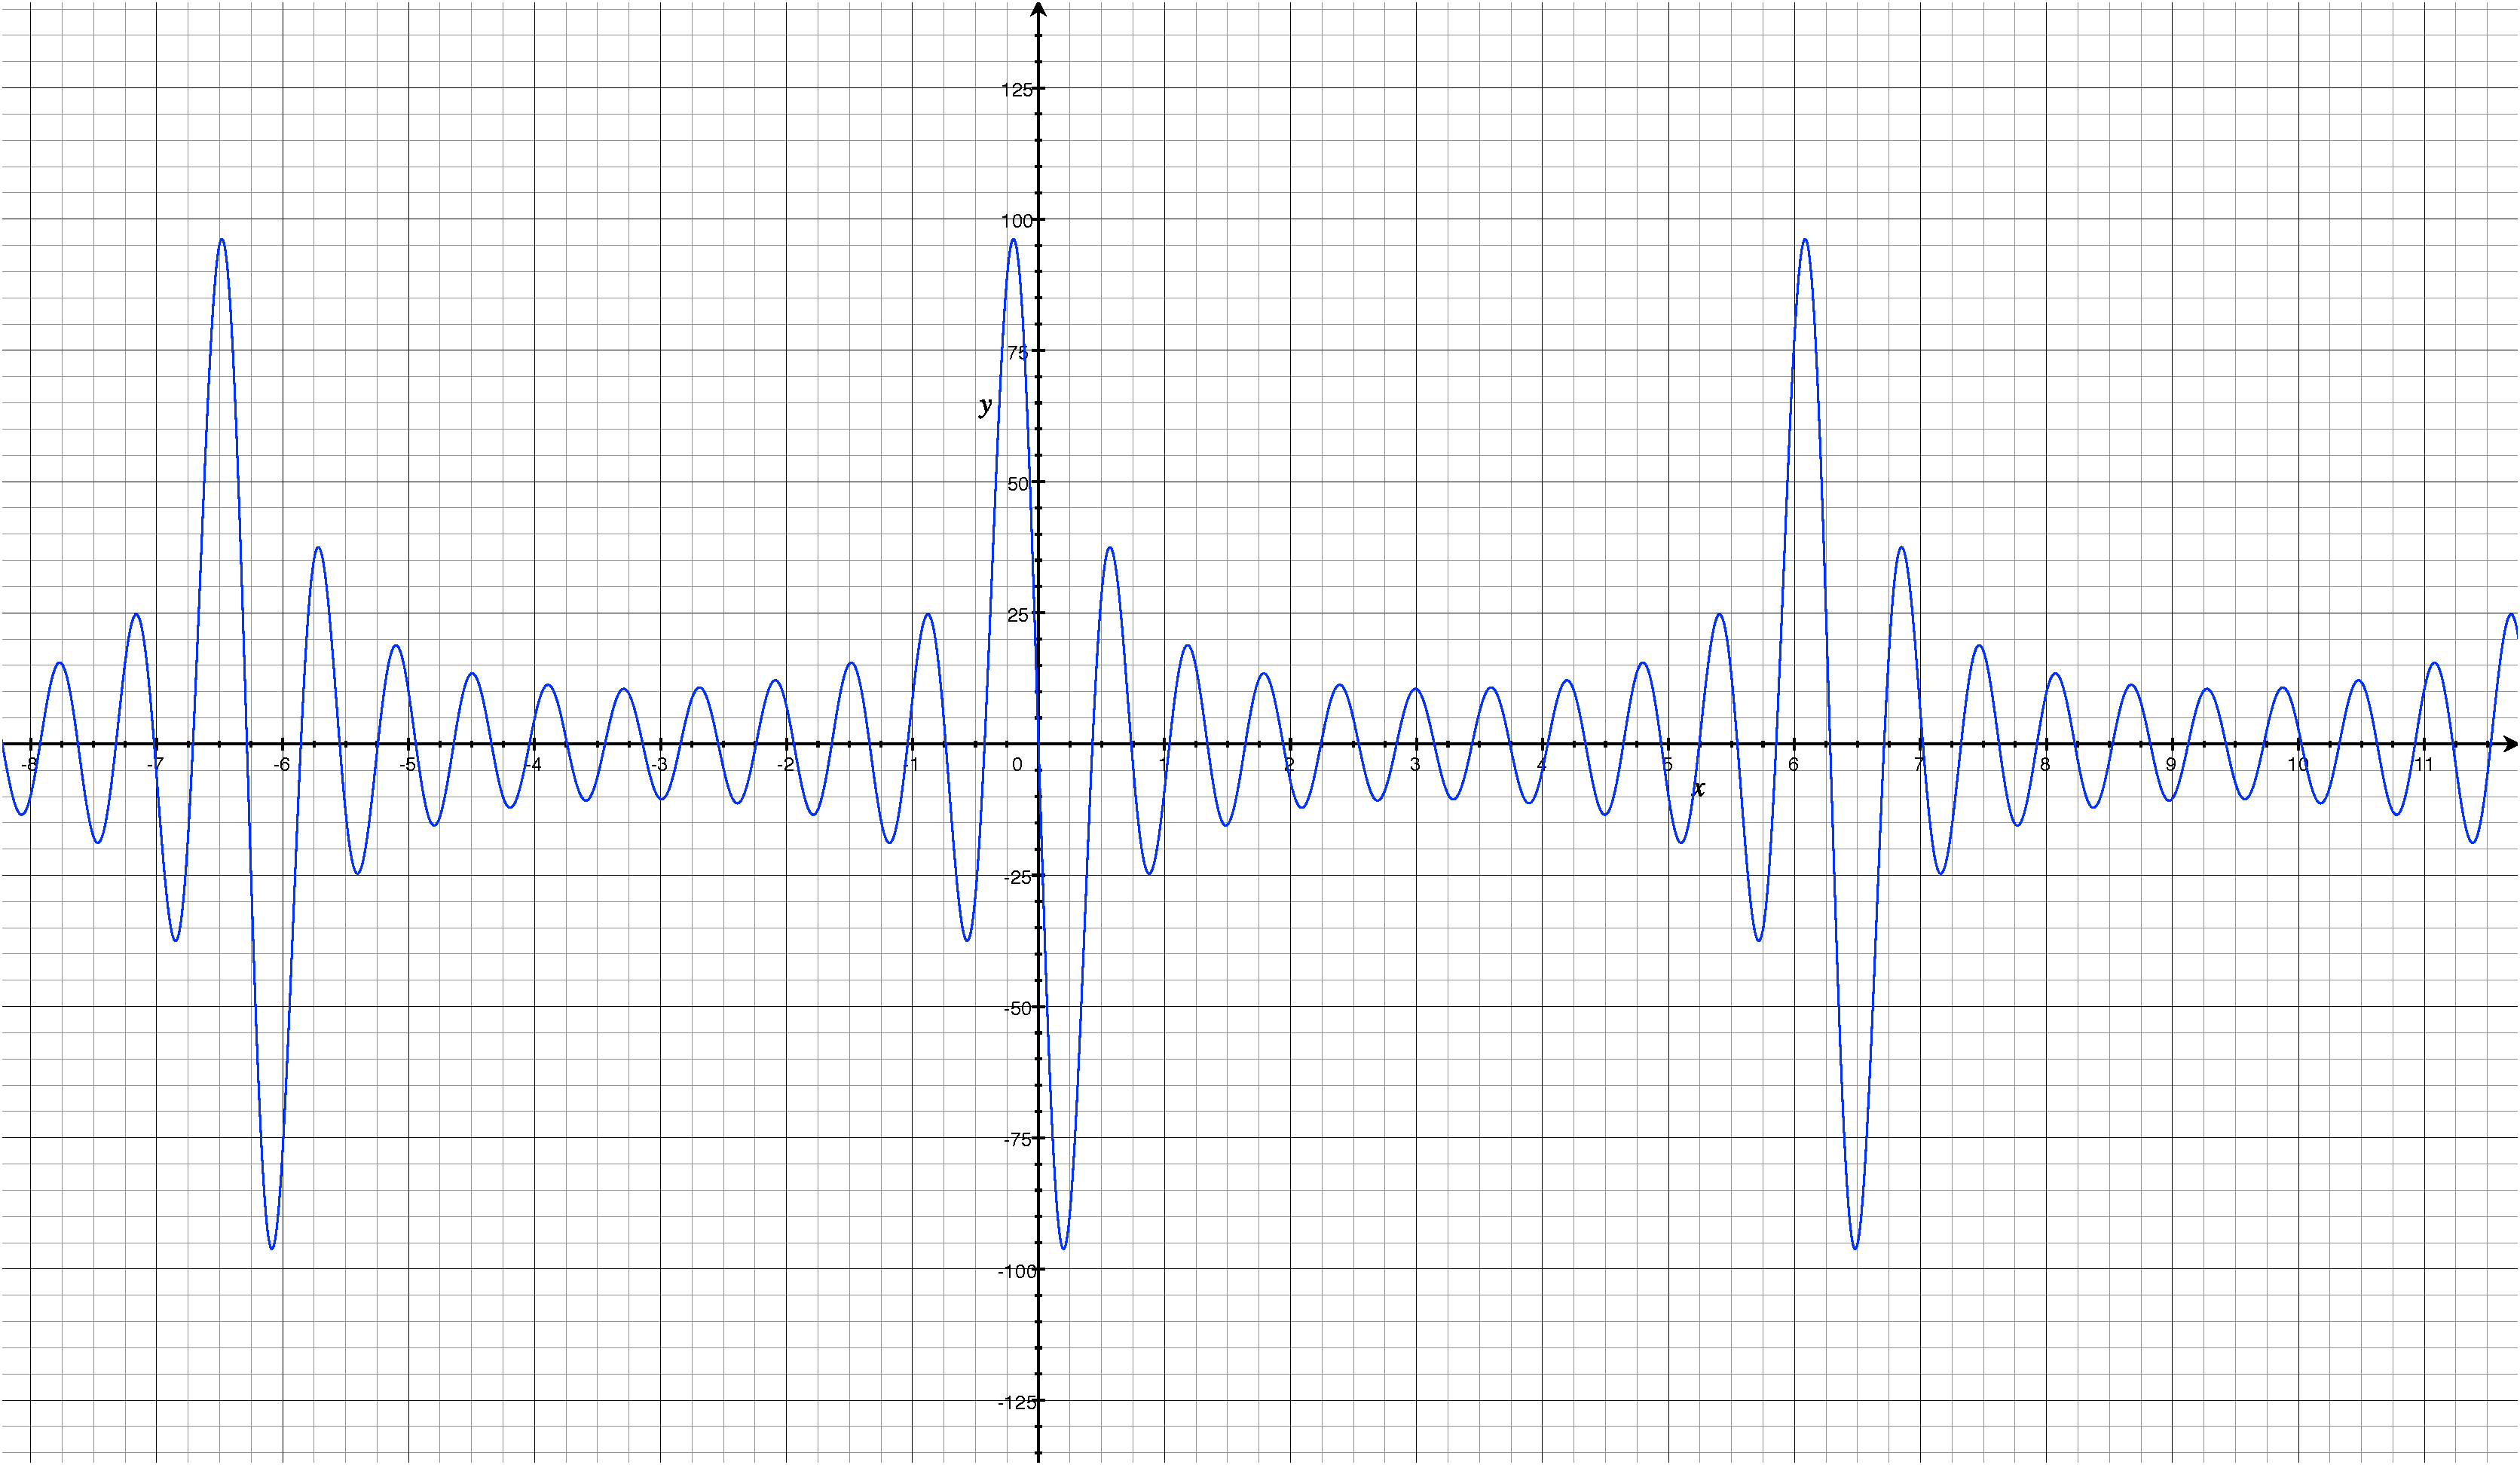
\includegraphics[width=0.8\textwidth]{Uebung3/Aufgabe_3_3_a_1.pdf} 
   \caption{$s(t)=\sum_{k=1}^n b_{k}sin(kt)=\sum_{k=1}^{n} jke^{jkt}-jke^{-jkt}, b_{k=-2k}, n=10$}
   \label{fig:3.3.a}
\end{figure}
\begin{figure}[h] %  figure placement: here, top, bottom, or page
   \centering
   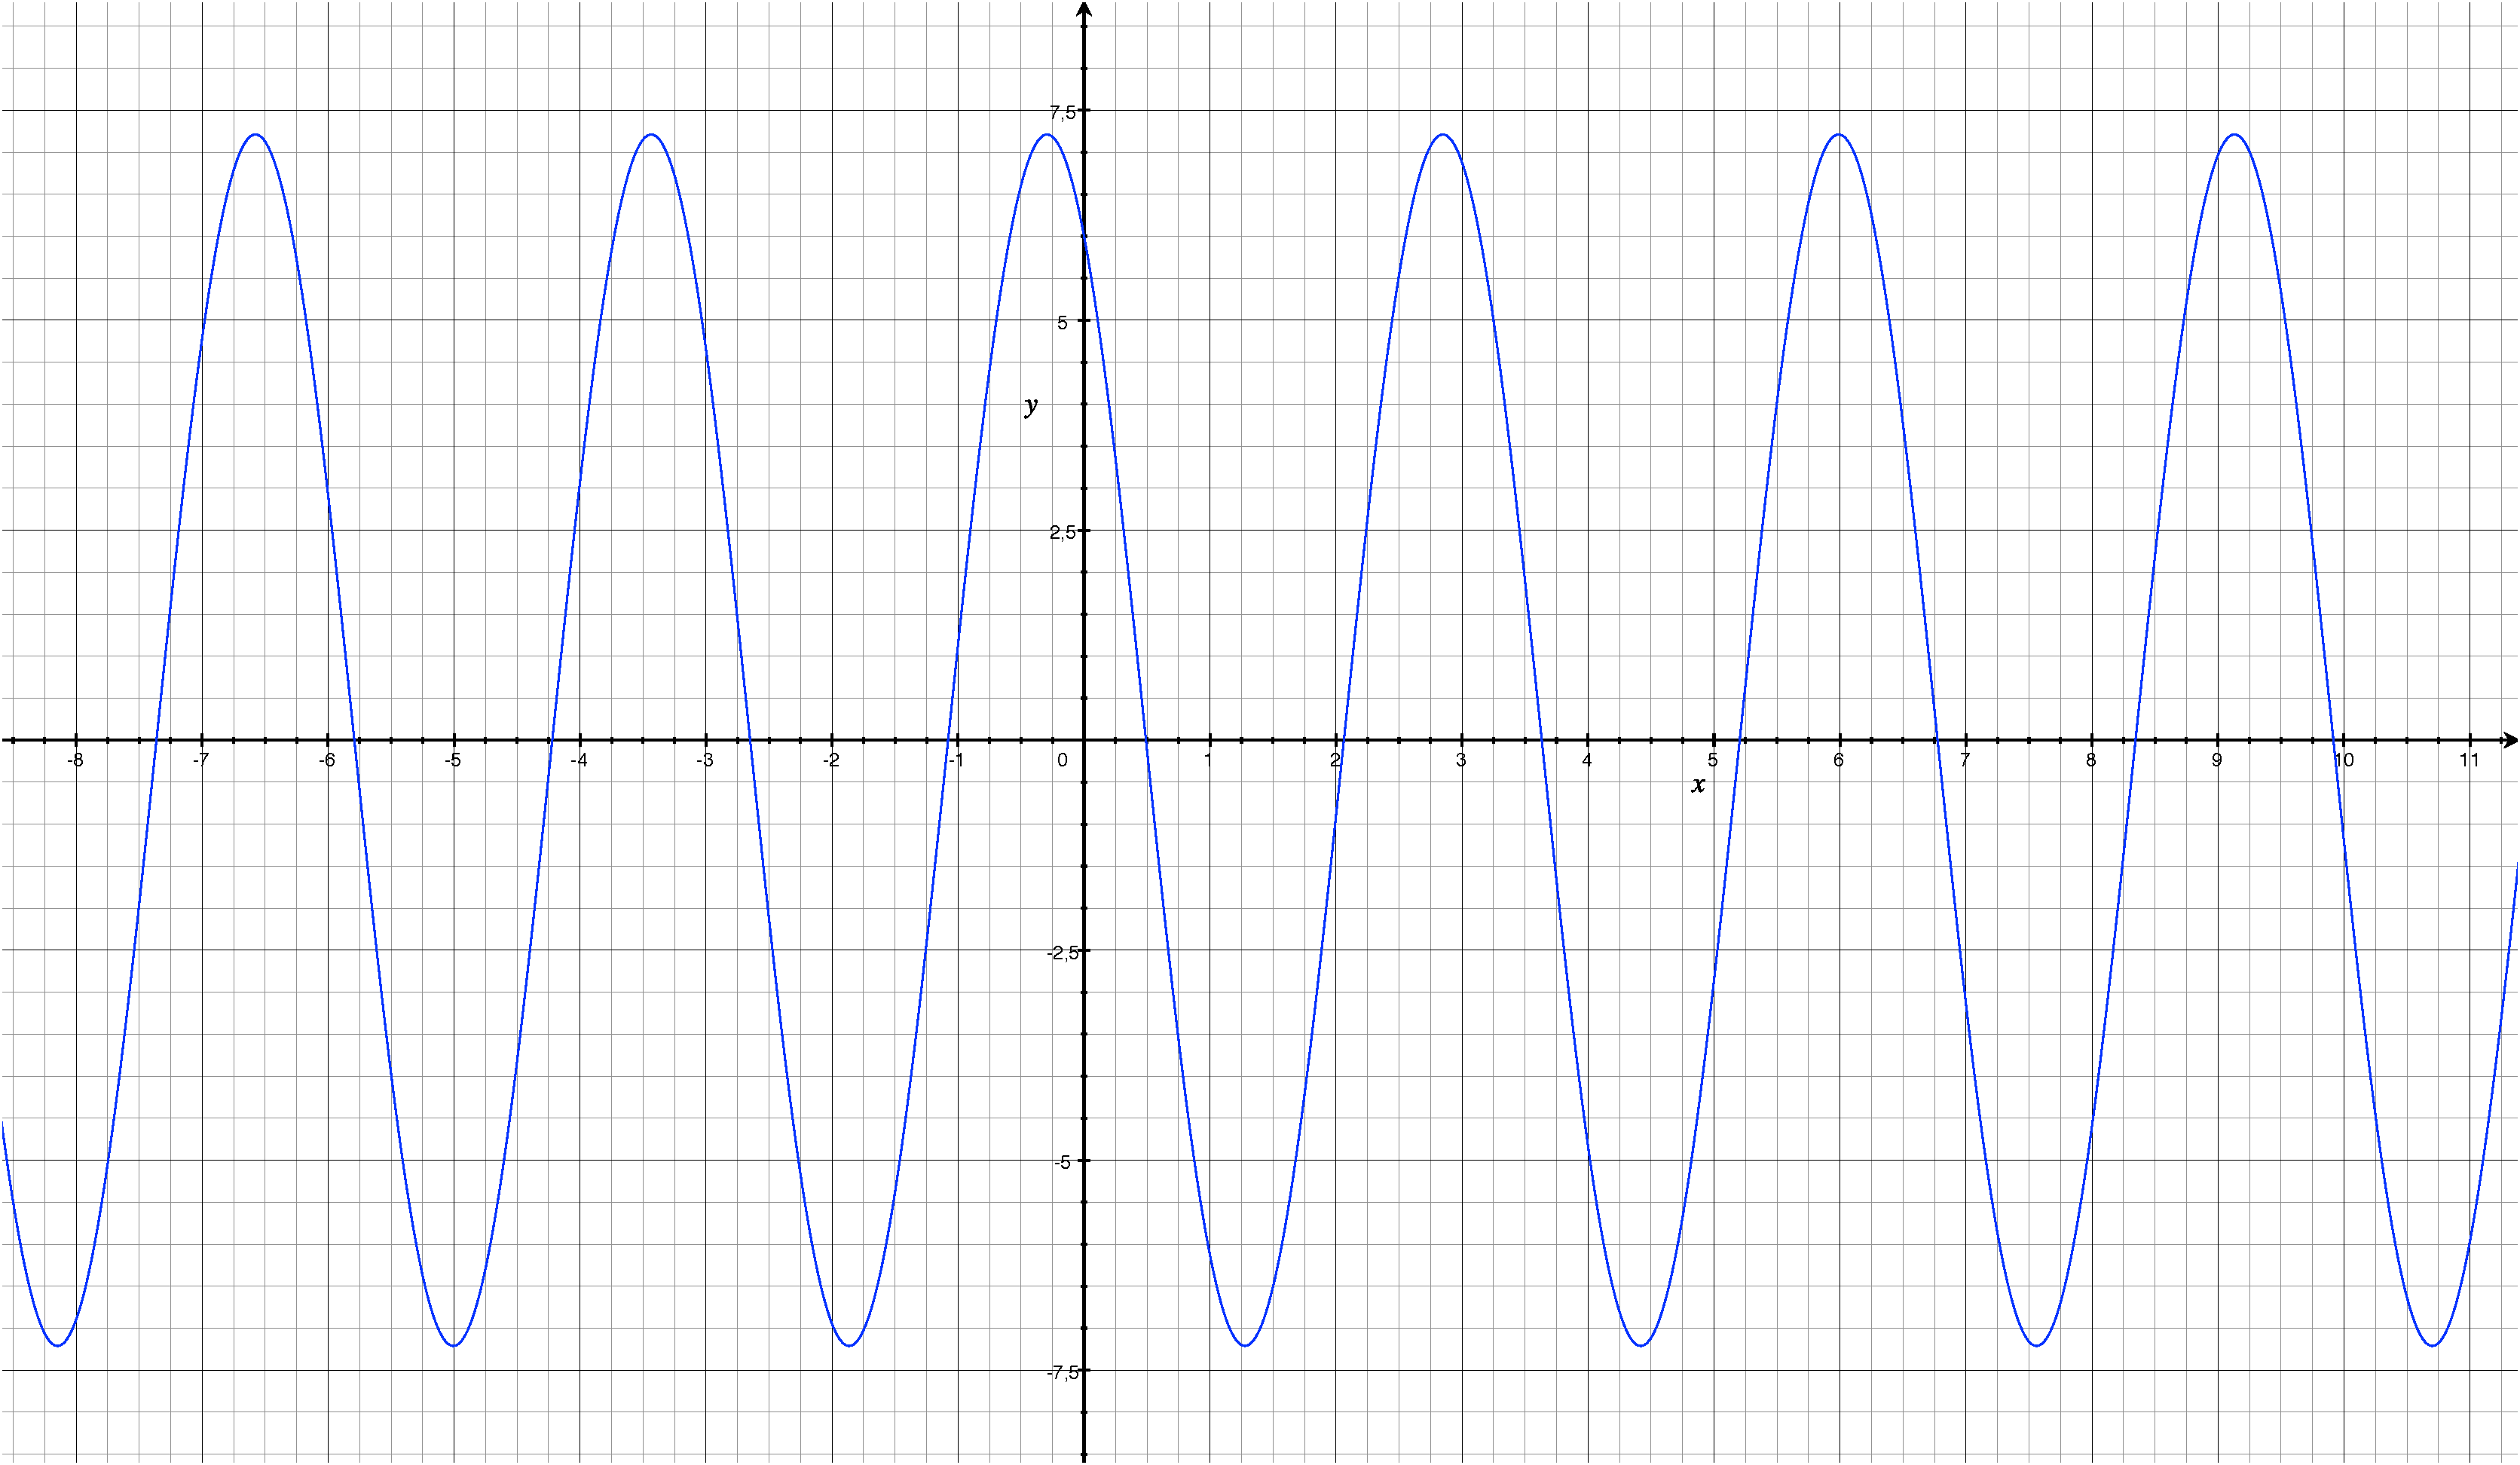
\includegraphics[width=0.8\textwidth]{Uebung3/Aufgabe_3_3_b.pdf} 
   \caption{$s(t)= 6cos(2t)-4sin(2t)=(3+2j)e^{j2t}+(3-2j)e^{-j2t}$}
   \label{fig:3.3.b}
\end{figure}